% Options for packages loaded elsewhere
\PassOptionsToPackage{unicode}{hyperref}
\PassOptionsToPackage{hyphens}{url}
%
\documentclass[
  12pt,
]{article}
\usepackage{lmodern}
\usepackage{amssymb,amsmath}
\usepackage{ifxetex,ifluatex}
\ifnum 0\ifxetex 1\fi\ifluatex 1\fi=0 % if pdftex
  \usepackage[T1]{fontenc}
  \usepackage[utf8]{inputenc}
  \usepackage{textcomp} % provide euro and other symbols
\else % if luatex or xetex
  \usepackage{unicode-math}
  \defaultfontfeatures{Scale=MatchLowercase}
  \defaultfontfeatures[\rmfamily]{Ligatures=TeX,Scale=1}
  \setmainfont[]{Times New Roman}
\fi
% Use upquote if available, for straight quotes in verbatim environments
\IfFileExists{upquote.sty}{\usepackage{upquote}}{}
\IfFileExists{microtype.sty}{% use microtype if available
  \usepackage[]{microtype}
  \UseMicrotypeSet[protrusion]{basicmath} % disable protrusion for tt fonts
}{}
\makeatletter
\@ifundefined{KOMAClassName}{% if non-KOMA class
  \IfFileExists{parskip.sty}{%
    \usepackage{parskip}
  }{% else
    \setlength{\parindent}{0pt}
    \setlength{\parskip}{6pt plus 2pt minus 1pt}}
}{% if KOMA class
  \KOMAoptions{parskip=half}}
\makeatother
\usepackage{xcolor}
\IfFileExists{xurl.sty}{\usepackage{xurl}}{} % add URL line breaks if available
\IfFileExists{bookmark.sty}{\usepackage{bookmark}}{\usepackage{hyperref}}
\hypersetup{
  pdftitle={Relationship Between Financial Data and Forest Coverage in 2018},
  pdfauthor={Ben Culberson, Emma DeAngeli, and Shana Shapiro},
  hidelinks,
  pdfcreator={LaTeX via pandoc}}
\urlstyle{same} % disable monospaced font for URLs
\usepackage[margin=2.54cm]{geometry}
\usepackage{longtable,booktabs}
% Correct order of tables after \paragraph or \subparagraph
\usepackage{etoolbox}
\makeatletter
\patchcmd\longtable{\par}{\if@noskipsec\mbox{}\fi\par}{}{}
\makeatother
% Allow footnotes in longtable head/foot
\IfFileExists{footnotehyper.sty}{\usepackage{footnotehyper}}{\usepackage{footnote}}
\makesavenoteenv{longtable}
\usepackage{graphicx,grffile}
\makeatletter
\def\maxwidth{\ifdim\Gin@nat@width>\linewidth\linewidth\else\Gin@nat@width\fi}
\def\maxheight{\ifdim\Gin@nat@height>\textheight\textheight\else\Gin@nat@height\fi}
\makeatother
% Scale images if necessary, so that they will not overflow the page
% margins by default, and it is still possible to overwrite the defaults
% using explicit options in \includegraphics[width, height, ...]{}
\setkeys{Gin}{width=\maxwidth,height=\maxheight,keepaspectratio}
% Set default figure placement to htbp
\makeatletter
\def\fps@figure{htbp}
\makeatother
\setlength{\emergencystretch}{3em} % prevent overfull lines
\providecommand{\tightlist}{%
  \setlength{\itemsep}{0pt}\setlength{\parskip}{0pt}}
\setcounter{secnumdepth}{5}
\usepackage{float}
\let\origfigure\figure
\let\endorigfigure\endfigure
\renewenvironment{figure}[1][2] {
    \expandafter\origfigure\expandafter[H]
} {
    \endorigfigure
}

\title{Relationship Between Financial Data and Forest Coverage in 2018}
\usepackage{etoolbox}
\makeatletter
\providecommand{\subtitle}[1]{% add subtitle to \maketitle
  \apptocmd{\@title}{\par {\large #1 \par}}{}{}
}
\makeatother
\subtitle{\url{https://github.com/emmadeangeli/Shapiro_DeAngeli_Culberson_ENV872_EDA_FinalProject.git}}
\author{Ben Culberson, Emma DeAngeli, and Shana Shapiro}
\date{}

\begin{document}
\maketitle

\newpage
\tableofcontents 
\newpage
\listoffigures
\newpage

\hypertarget{rationale-and-research-questions}{%
\section{Rationale and Research
Questions}\label{rationale-and-research-questions}}

We were initially interested in whether climate financing correlated to
environmental health in various countries. However, we could not find
enough data to lead to a robust analysis. Instead, we are looking into
whether different financial indicators (in as many countries as we could
find) lead specifically to forest coverage. In our project, we are using
forest coverage as a proxy for environmental health. Developed countries
may have the luxury of being able to preserve their forests. We were
particularly interested in seeing if other financial indicators related
to forest coverage. Our main research question was ``do financial
indicators correlate to forest coverage for different countries in
2018?'' Therefore, our hypotheses are the following:

\[H_0:\] There are no financial indicators or combination of financial
indicators that correlate to forest coverage. \[H_a:\] There is at least
one financial indicator or combination of financial indicators that
correlates to forest coverage.

\newpage

\hypertarget{dataset-information}{%
\section{Dataset Information}\label{dataset-information}}

We pulled our data from three databases on the World Bank website:
Global Financial Development, Global Economic Monitor, and Country
Climate and Development Report. The first two have variables related to
financial and economic data while the third has variables related to
climate and development. After transposing the data from the World Bank
Website such that each variable has its own column rather than its own
row, we joined data from the three sets with a leftjoin() command and
then filtered the resulting data set with a na.omit() command. Finally
we were left with four selected variables to analyze in the year 2018:

Table 1. Variables

\begin{longtable}[]{@{}ll@{}}
\toprule
\begin{minipage}[b]{0.54\columnwidth}\raggedright
Dataset\strut
\end{minipage} & \begin{minipage}[b]{0.40\columnwidth}\raggedright
Description\strut
\end{minipage}\tabularnewline
\midrule
\endhead
\begin{minipage}[t]{0.54\columnwidth}\raggedright
Central Bank Assets to GDP (\%)\strut
\end{minipage} & \begin{minipage}[t]{0.40\columnwidth}\raggedright
This variable is equal to a given country's central bank assets divided
by its GDP for the year 2018\strut
\end{minipage}\tabularnewline
\begin{minipage}[t]{0.54\columnwidth}\raggedright
Domestic Credit to Private Sector (\% of GDP)\strut
\end{minipage} & \begin{minipage}[t]{0.40\columnwidth}\raggedright
This variable is equal to the amount of private investment in a given
countries debt divided by that countries GDP for the year 2018\strut
\end{minipage}\tabularnewline
\begin{minipage}[t]{0.54\columnwidth}\raggedright
Domestic Reserves (Million US\$)\strut
\end{minipage} & \begin{minipage}[t]{0.40\columnwidth}\raggedright
This variable is equal to a given country's monetary reserves held by
its central bank in million USD for the year 2018\strut
\end{minipage}\tabularnewline
\begin{minipage}[t]{0.54\columnwidth}\raggedright
\textbf{Dependent variable:}\strut
\end{minipage} & \begin{minipage}[t]{0.40\columnwidth}\raggedright
Share of surface occupied by forest (\%)\strut
\end{minipage}\tabularnewline
\bottomrule
\end{longtable}

\newpage

\hypertarget{exploratory-analysis}{%
\section{Exploratory Analysis}\label{exploratory-analysis}}

\hypertarget{individual-linear-regressions-with-each-financial-variable}{%
\subsection{Individual Linear Regressions with Each Financial
Variable}\label{individual-linear-regressions-with-each-financial-variable}}

\begin{verbatim}
## 
## Call:
## lm(formula = Forest_Share_of_Surface ~ credit.to.private, data = finance_forests.df)
## 
## Residuals:
##     Min      1Q  Median      3Q     Max 
## -33.419 -19.682  -1.393  13.912  61.045 
## 
## Coefficients:
##                   Estimate Std. Error t value Pr(>|t|)    
## (Intercept)       31.91587    4.05139   7.878 4.88e-12 ***
## credit.to.private  0.01868    0.05225   0.358    0.721    
## ---
## Signif. codes:  0 '***' 0.001 '**' 0.01 '*' 0.05 '.' 0.1 ' ' 1
## 
## Residual standard error: 21.58 on 97 degrees of freedom
## Multiple R-squared:  0.001317,   Adjusted R-squared:  -0.008979 
## F-statistic: 0.1279 on 1 and 97 DF,  p-value: 0.7214
\end{verbatim}

\begin{verbatim}
## 
## Call:
## lm(formula = Forest_Share_of_Surface ~ assets.to.gdp, data = finance_forests.df)
## 
## Residuals:
##     Min      1Q  Median      3Q     Max 
## -33.964 -16.681  -2.608  14.229  56.839 
## 
## Coefficients:
##               Estimate Std. Error t value Pr(>|t|)    
## (Intercept)    29.9110     2.4583  12.167   <2e-16 ***
## assets.to.gdp   0.5564     0.2197   2.532   0.0129 *  
## ---
## Signif. codes:  0 '***' 0.001 '**' 0.01 '*' 0.05 '.' 0.1 ' ' 1
## 
## Residual standard error: 20.91 on 97 degrees of freedom
## Multiple R-squared:  0.062,  Adjusted R-squared:  0.05233 
## F-statistic: 6.411 on 1 and 97 DF,  p-value: 0.01295
\end{verbatim}

\begin{verbatim}
## 
## Call:
## lm(formula = Forest_Share_of_Surface ~ Reserves, data = finance_forests.df)
## 
## Residuals:
##     Min      1Q  Median      3Q     Max 
## -33.189 -18.793  -0.428  14.346  60.609 
## 
## Coefficients:
##              Estimate Std. Error t value Pr(>|t|)    
## (Intercept) 3.303e+01  2.241e+00  14.742   <2e-16 ***
## Reserves    1.206e-06  6.431e-06   0.188    0.852    
## ---
## Signif. codes:  0 '***' 0.001 '**' 0.01 '*' 0.05 '.' 0.1 ' ' 1
## 
## Residual standard error: 21.59 on 97 degrees of freedom
## Multiple R-squared:  0.0003626,  Adjusted R-squared:  -0.009943 
## F-statistic: 0.03518 on 1 and 97 DF,  p-value: 0.8516
\end{verbatim}

\hypertarget{plots-of-share-of-surface-occupied-by-forest-on-all-3-financial-variables}{%
\subsection{Plots of Share of Surface Occupied by Forest on all 3
financial
variables}\label{plots-of-share-of-surface-occupied-by-forest-on-all-3-financial-variables}}

\begin{figure}
\centering
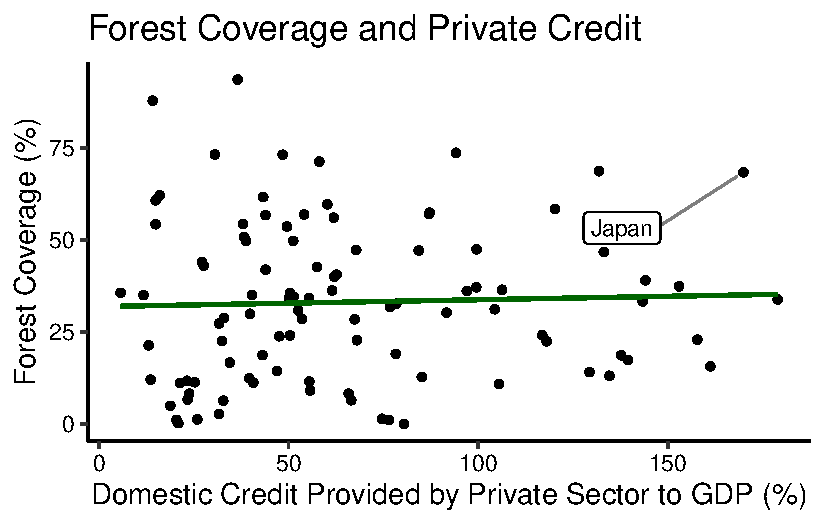
\includegraphics{CulbersonDeAngeliShapiro_ENV872_Project_files/figure-latex/unnamed-chunk-1-1.pdf}
\caption{Forest Coverage and Private Credit}
\end{figure}

\begin{figure}
\centering
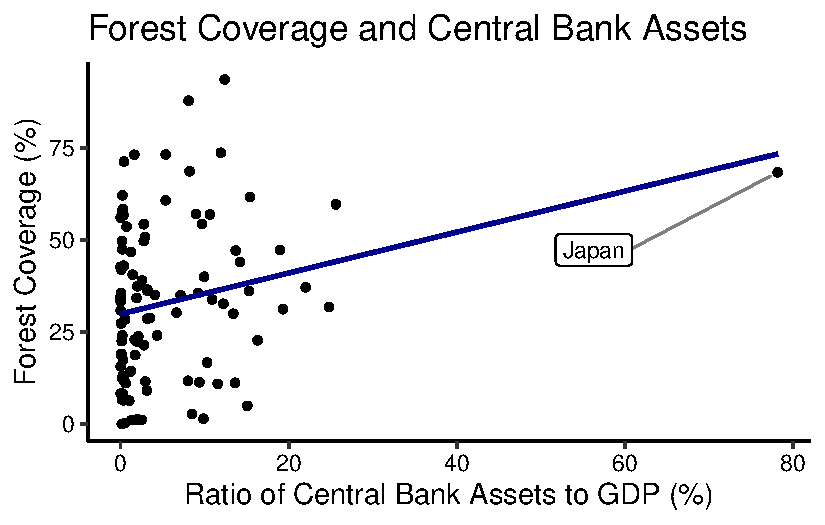
\includegraphics{CulbersonDeAngeliShapiro_ENV872_Project_files/figure-latex/fccba-1.pdf}
\caption{Forest Coverage and Central Bank Assets}
\end{figure}

\begin{figure}
\centering
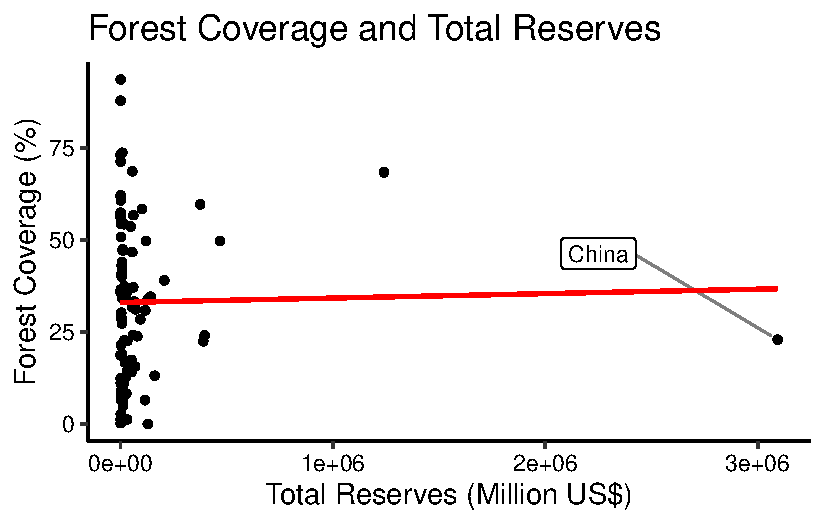
\includegraphics{CulbersonDeAngeliShapiro_ENV872_Project_files/figure-latex/unnamed-chunk-2-1.pdf}
\caption{Forest Coverage and Total Reserves}
\end{figure}

\newpage

\hypertarget{residuals-and-errors}{%
\subsection{Residuals and Errors}\label{residuals-and-errors}}

\begin{figure}
\centering
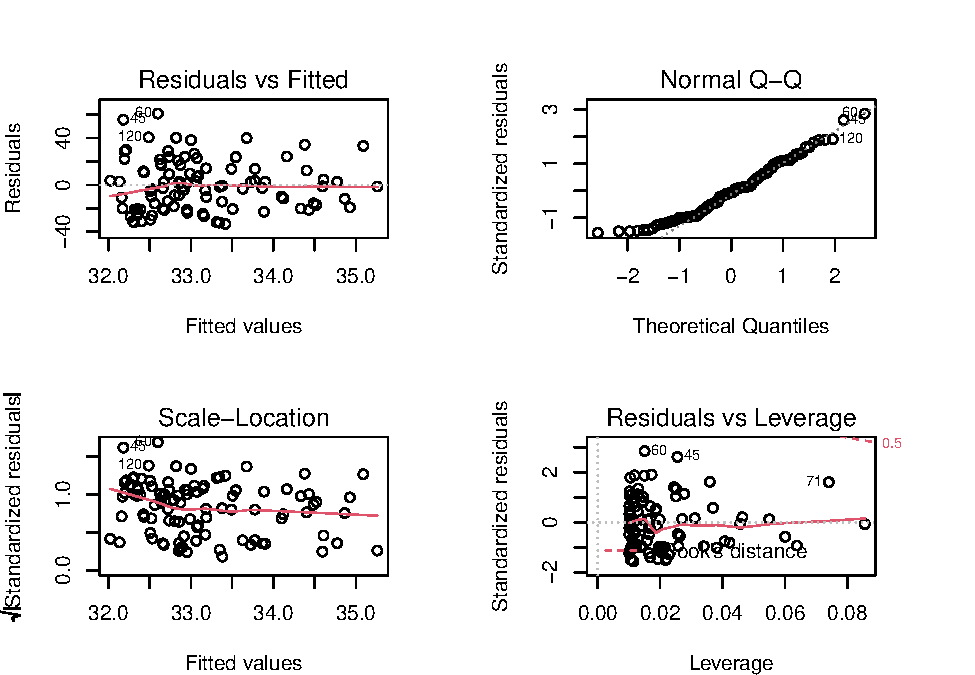
\includegraphics{CulbersonDeAngeliShapiro_ENV872_Project_files/figure-latex/unnamed-chunk-3-1.pdf}
\caption{Residuals from Private Credit Regression}
\end{figure}

\begin{figure}
\centering
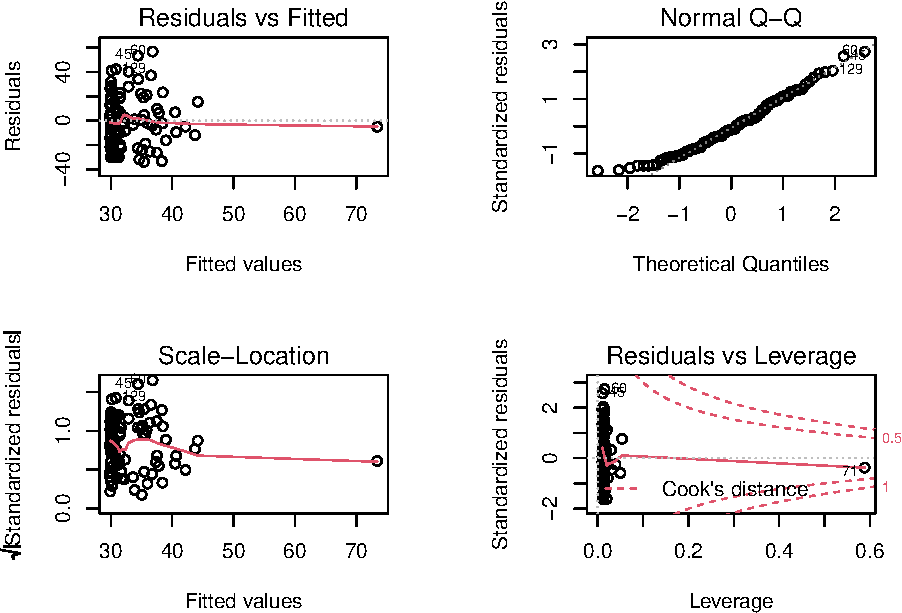
\includegraphics{CulbersonDeAngeliShapiro_ENV872_Project_files/figure-latex/unnamed-chunk-4-1.pdf}
\caption{Residuals from Central Bank Assets to GDP Regression}
\end{figure}

\begin{figure}
\centering
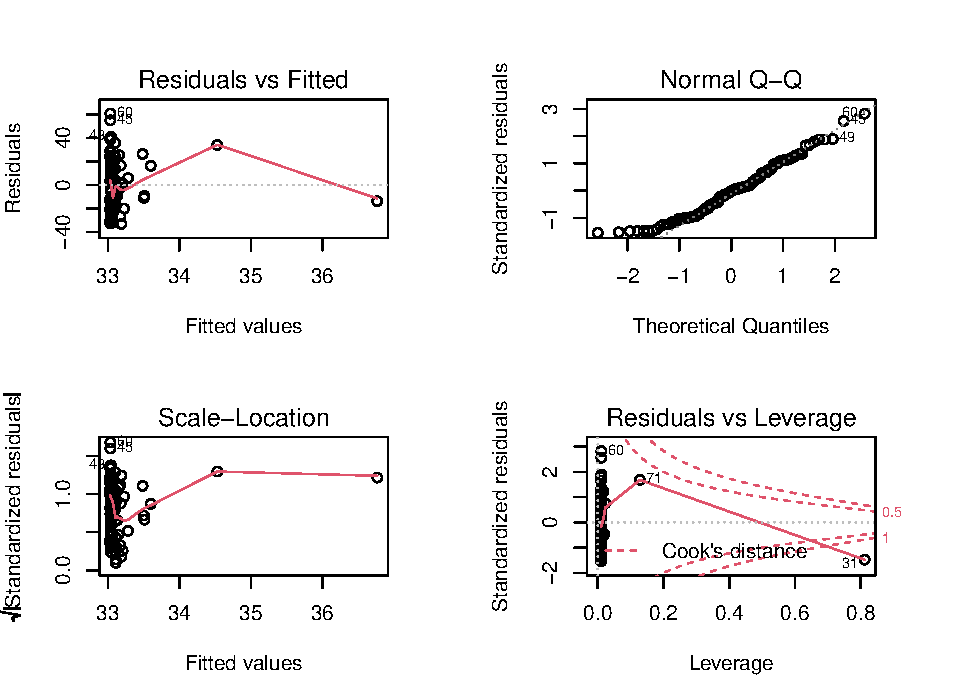
\includegraphics{CulbersonDeAngeliShapiro_ENV872_Project_files/figure-latex/unnamed-chunk-5-1.pdf}
\caption{Residuals from Total Reserves Regression}
\end{figure}

\newpage

\hypertarget{creating-a-multivariate-linear-model}{%
\subsection{Creating a Multivariate Linear
Model}\label{creating-a-multivariate-linear-model}}

Akaike information criterion and step test, leading to the final model:

\begin{verbatim}
## Start:  AIC=607.79
## Forest_Share_of_Surface ~ credit.to.private + assets.to.gdp + 
##     Reserves
## 
##                     Df Sum of Sq   RSS    AIC
## - credit.to.private  1      0.40 42345 605.79
## - Reserves           1     69.15 42413 605.95
## <none>                           42344 607.79
## - assets.to.gdp      1   2815.90 45160 612.16
## 
## Step:  AIC=605.79
## Forest_Share_of_Surface ~ assets.to.gdp + Reserves
## 
##                 Df Sum of Sq   RSS    AIC
## - Reserves       1     73.52 42418 603.96
## <none>                       42345 605.79
## - assets.to.gdp  1   2860.66 45205 610.26
## 
## Step:  AIC=603.96
## Forest_Share_of_Surface ~ assets.to.gdp
## 
##                 Df Sum of Sq   RSS    AIC
## <none>                       42418 603.96
## - assets.to.gdp  1    2803.5 45222 608.30
\end{verbatim}

\begin{verbatim}
## 
## Call:
## lm(formula = Forest_Share_of_Surface ~ assets.to.gdp, data = finance_forests.df)
## 
## Coefficients:
##   (Intercept)  assets.to.gdp  
##       29.9110         0.5564
\end{verbatim}

\begin{verbatim}
## 
## Call:
## lm(formula = Forest_Share_of_Surface ~ credit.to.private + assets.to.gdp + 
##     Reserves, data = finance_forests.df)
## 
## Residuals:
##     Min      1Q  Median      3Q     Max 
## -34.296 -16.685  -2.649  14.391  56.515 
## 
## Coefficients:
##                     Estimate Std. Error t value Pr(>|t|)    
## (Intercept)        2.992e+01  4.103e+00   7.292 9.07e-11 ***
## credit.to.private  1.639e-03  5.499e-02   0.030   0.9763    
## assets.to.gdp      5.773e-01  2.297e-01   2.513   0.0136 *  
## Reserves          -2.693e-06  6.837e-06  -0.394   0.6945    
## ---
## Signif. codes:  0 '***' 0.001 '**' 0.01 '*' 0.05 '.' 0.1 ' ' 1
## 
## Residual standard error: 21.11 on 95 degrees of freedom
## Multiple R-squared:  0.06363,    Adjusted R-squared:  0.03406 
## F-statistic: 2.152 on 3 and 95 DF,  p-value: 0.09883
\end{verbatim}

\begin{verbatim}
## 
## Call:
## lm(formula = Forest_Share_of_Surface ~ assets.to.gdp, data = finance_forests.df)
## 
## Residuals:
##     Min      1Q  Median      3Q     Max 
## -33.964 -16.681  -2.608  14.229  56.839 
## 
## Coefficients:
##               Estimate Std. Error t value Pr(>|t|)    
## (Intercept)    29.9110     2.4583  12.167   <2e-16 ***
## assets.to.gdp   0.5564     0.2197   2.532   0.0129 *  
## ---
## Signif. codes:  0 '***' 0.001 '**' 0.01 '*' 0.05 '.' 0.1 ' ' 1
## 
## Residual standard error: 20.91 on 97 degrees of freedom
## Multiple R-squared:  0.062,  Adjusted R-squared:  0.05233 
## F-statistic: 6.411 on 1 and 97 DF,  p-value: 0.01295
\end{verbatim}

\begin{figure}
\centering
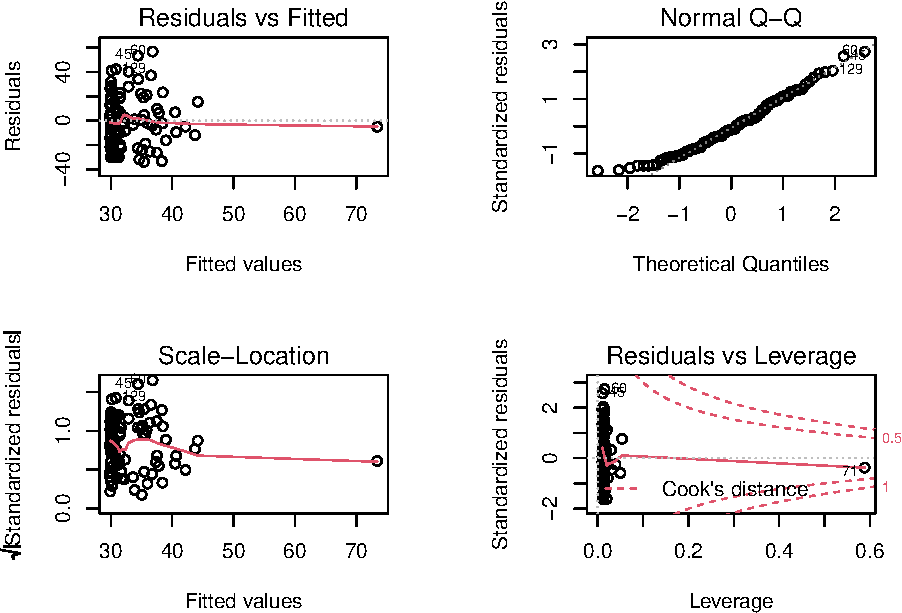
\includegraphics{CulbersonDeAngeliShapiro_ENV872_Project_files/figure-latex/unnamed-chunk-6-1.pdf}
\caption{Residuals from Multivariate Regression}
\end{figure}

ANOVA test:

\begin{verbatim}
##               Df Sum Sq Mean Sq F value Pr(>F)  
## assets.to.gdp  1   2804  2803.5   6.411 0.0129 *
## Residuals     97  42418   437.3                 
## ---
## Signif. codes:  0 '***' 0.001 '**' 0.01 '*' 0.05 '.' 0.1 ' ' 1
\end{verbatim}

\newpage

\hypertarget{analysis}{%
\section{Analysis}\label{analysis}}

After running 3 individual linear regressions with each of the financial
variables we selected, only the regression with the Central Bank Assets
to GDP variable had statistically significant p-value at 0.01295. The
adjusted R-squared for regression case was 0.052, meaning that the
linear model only explains roughly 5\% of the variation in our dependent
variable, Share of Surface Occupied by Forest (\%). Despite this low
adjusted R-squared, the output from this regression tells us that a 1\%
increase in the Assets to GDP Ratio of a given country is correlated
with a 0.56\% increase in the share of that country's surface covered by
forest. The other two linear regressions had no statistically
significant explanatory variables and had adjusted R-squared values that
were close to zero so we choose not to interpret their coefficients.

After running these linear regressions, we plotted the Share of Surface
Occupied by Forest on each explanatory financial variable in 3 separate
scatterplots (Figures 1-3) . On each scatterplot, we also plotted the
fitted linear regression. In all three plots, it becomes clear the low
adjusted R-squared values from our regressions were appropriate. The
fitted linear regressions do not appear to explain much of the variation
in our dependent variable. In the case of the Forest Coverage and
Private Credit (Figure 1) and Forest Coverage (Figure 2) and Total
Reserves (Figure 3) plots, the linear fit does an exceptionally poor job
of relating the explanatory variables to the Share of Surface Occupied
by Forest dependent variable. Only for the Forest Coverage and Central
Bank Assets plot (Figure 2) does the fitted linear regression seem to
make sense and even in this case, there is stil a considerable amount of
the data that the fitted regression does not explain.

From the residual plots of these 3 individual linear regressions, we see
that Figures 5 and 6 (for the Total Reserves explanatory variable and
the Assets to GDP explanatory variable, respectively) had residuals
concentrated highly on the left hand side of the plots, and had fitted
lines that did little to minimize the magnitude of these residuals.
These two observations indicate that our models are not well fitted, and
the corresponding adjusted-R squared values align with that indication.
Figure 4 on the other hand (for the Domestic Credit to Private Sector
explanatory variable), seemed to indicate a better fitting model. In
this case, there is less drastic asymmetry in the residuals and the
residuals are much closer to zero than the other two regressions.
However, the output for this single variable regression still shows that
the model does not do a good job of fitting the data.

When we put all three explanatory financial variables together in a
multivariate regression, we use the Akaike's Information Criterion (AIC)
to select which variables are useful. After just 3 steps, the AIC tells
us that the only needed explanatory financial variable is the Central
Bank Assets to GDP ratio. In other words, the Total Reserves explanatory
variable and the Domestic Credit to Private Sector explanatory variable
are not terribly useful in modeling the Share Forest Coverage, possibly
because they co-vary with other explanatory variables. The full
multivariate linear model with all 3 financial variables still has an
F-statistic that is somewhat statistically significant at the 0.1 level,
but the regression with only the Central Bank Assets to GDP ratio has an
F-statistic significant at the 0.05 level (equal to the p-value of the
Central Bank Assets to GDP variable). Our integration of our final model
then, is equivalent to the interpretation of single variable regression
for Central Bank Assets to GDP (they are the same model). A 1\% increase
in the Assets to GDP Ratio of a given country is correlated with a
0.56\% increase in the share of that country's surface covered by
forest. Any change in our other explanatory variables has no
statistically significant correlation with the Share of Forest Coverage
according to the models we run. Furthermore, the residuals of this final
regression are equivalent to the residuals of our Central Bank Assets to
GDP single variable regression (see Figures 7 and 5), so we do not
observe anything different from the plots in Figure 7.

\hypertarget{question-do-financial-indicators-correlate-to-forest-coverage-for-different-countries-in-2018}{%
\subsection{Question: Do financial indicators correlate to forest
coverage for different countries in
2018?}\label{question-do-financial-indicators-correlate-to-forest-coverage-for-different-countries-in-2018}}

As stated in our analysis, at least the Central Bank Assets to GDP has a
statistically significant correlation with Share of Forest Coverage.

\newpage

\hypertarget{summary-and-conclusions}{%
\section{Summary and Conclusions}\label{summary-and-conclusions}}

In summary, we reject the null hypothesis at the 0.05 level that there
are no financial indicators or combination of financial indicators that
correlate to forest coverage. Through our multiple linear regression, we
find that the Central Bank Assets to GDP does have a statistically
significant correlation with Share of Forest Coverage (p = 0.0129).

With our result, we can answer that yes, financial indicators correlate
with various countries' forest coverage in 2018. While there is a
statistically significant correlation, there are limitations to our
analysis and we cannot reliably conclude where the causation of the
correlation originates. Our analysis does not consider the exhaustive
list of variables contributing to a country's forest cover, but it does
provide some insight into the statistical relationship between financial
indicators and environmental variables. Further research including
additional financial indicators or environmental responses may be
warranted.

\end{document}
